\chapter{Testing}
In this chapter we will be talking about the different techniques that we have employed to test the different aspects of the system.
We will first be talking about the different kind of unit tests that we have written.
These tests provide for a basic code coverage.
After this we will be talking about what kind integration tests we have performed to ensure the connection between the different components.
Lastly we will be talking about the acceptance tests that were performed.

\section{Testing methods during the implementation phase}
\subsection{Unit testing}
During the implementation phase a feature is only complete when it is fully tested.
This is done by running the system and testing it by the programmer, but also done by running automated tests.
These automated tests are required for achieving a good code coverage and for ensuring the code to work appropriately.
The tests that are written for other features will be always run after the feature has been merged.
This ensures that other features that may change the working of the code does not let the tests fail.
So all the features that were already in the system will still work even after the merging of the new feature.

In figure~\ref{testresulttrenddev} you can see the increasing amount of tests that increase with each pull request that has been merged with the development branch.
\begin{figure}[h]
    \centering
    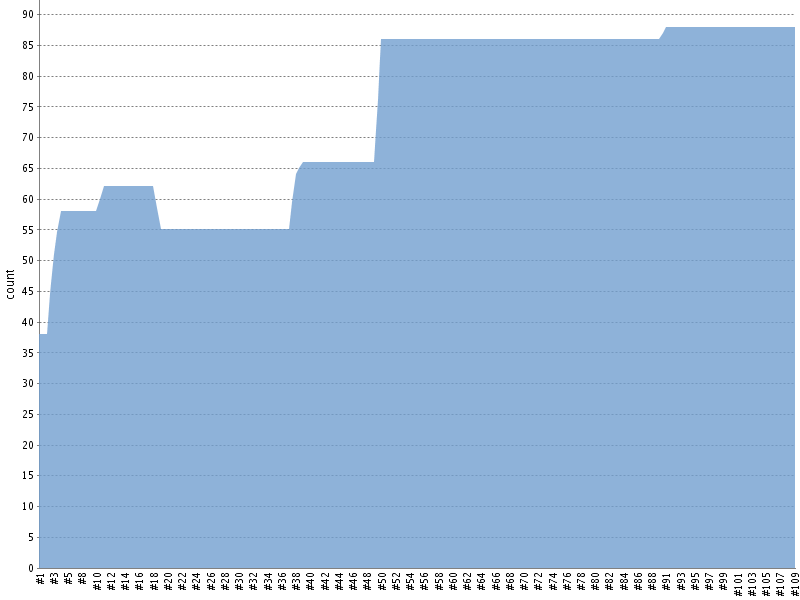
\includegraphics[width=\textwidth]{images/TestresultTrendDev2}
    \caption{Amount of tests per build}
    \label{testresulttrenddev}
\end{figure}

In figure~\ref{testresulttrendpullrequest} you can see the increasing amount of tests of the different pull requests that have been made.
In this image you can clearly see that when sometimes when a new feature is added, some tests start to fail.
Due to our continuous integration we could spot the errors early and make sure that they are fixed before merging with the development branch.

\begin{figure}[h]
    \centering
    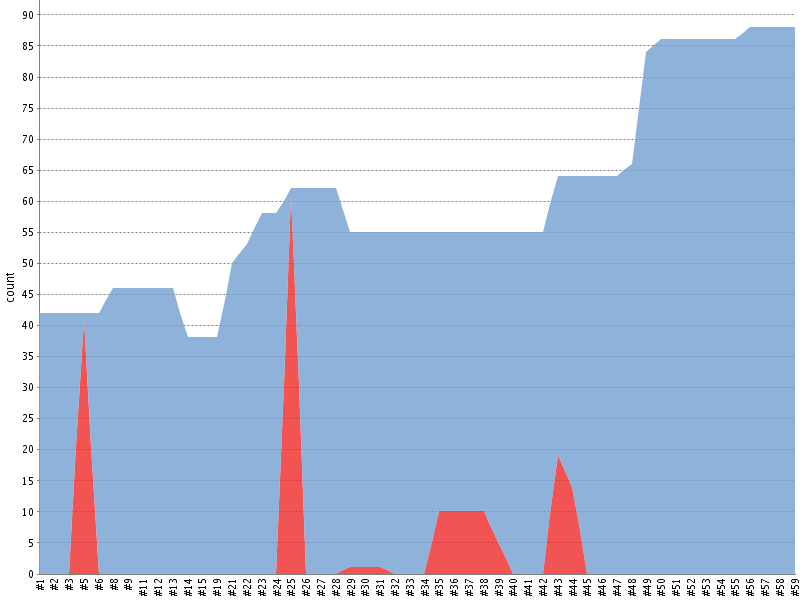
\includegraphics[width=\textwidth]{images/TestresultTrendPullRequests}
    \caption{Amount of tests per build of a pull request}
    \label{testresulttrendpullrequest}
\end{figure}

Figure~\ref{testresulttrendpullrequest} shows how not every pull request is without errors.
All of these errors first had to be resolved before the pull request could be merged.\\

Figure~\ref{codecoveragetrenddev} depicts the code coverage achieved by the tests.
The goal is to have the code coverage percentages to be around a certain percentage during the entire implementation.
One could argue that a 100\% code coverage is desired, but some features are quite trivial and don't need a 100\% code coverage.
Next to this is the fact that some plugins, in our case the eBean plugin, generates code for classes.
This generated code is not something we need to test since it is not written by us.\\

\begin{figure}[h]
    \centering
    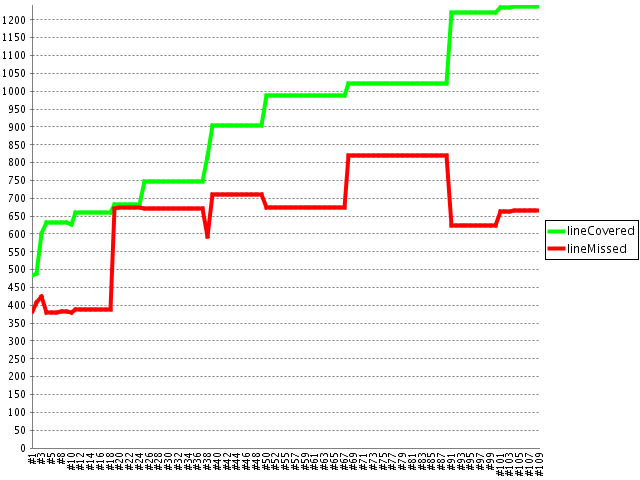
\includegraphics[width=\textwidth]{images/CodeCoverageTrendDev2}
    \caption{Code coverage trend for the development branch}
    \label{codecoveragetrenddev}
\end{figure}

We also underestimated the complexity of some features and thus did not wrote the tests for all cases with the first pull request of those features.
In that first basic implementation some of the cases were already implemented in part of the system but not actually called upon and made available from the front end.
We thus decided to first create a pull request for a basic version and thus split up the amount of changes.
Later, when the feature was further implemented, we added tests that would test these extra cases.

\subsection{Integration testing}
Everything a pull request was made, the changes were checked by a member of the team that wasn't the one requesting the merge.
This ensured that the changes made reflected the feature that was selected to be implemented.
The member of the team to check the code asked questions about some changes and checked if complex functions could be made more efficient.
Although we use checkstyle and findbugs to perform code analysis, they do not find everything.
So there is much value to achieve with a member of the team checking the code.

In figure~\ref{pullrequest-example} you can see an example of a pull request and how a team member commented on a part of the code.
The requesting team member responded on the issue and argued why he choose the implementation.

\begin{figure}[h]
    \centering
    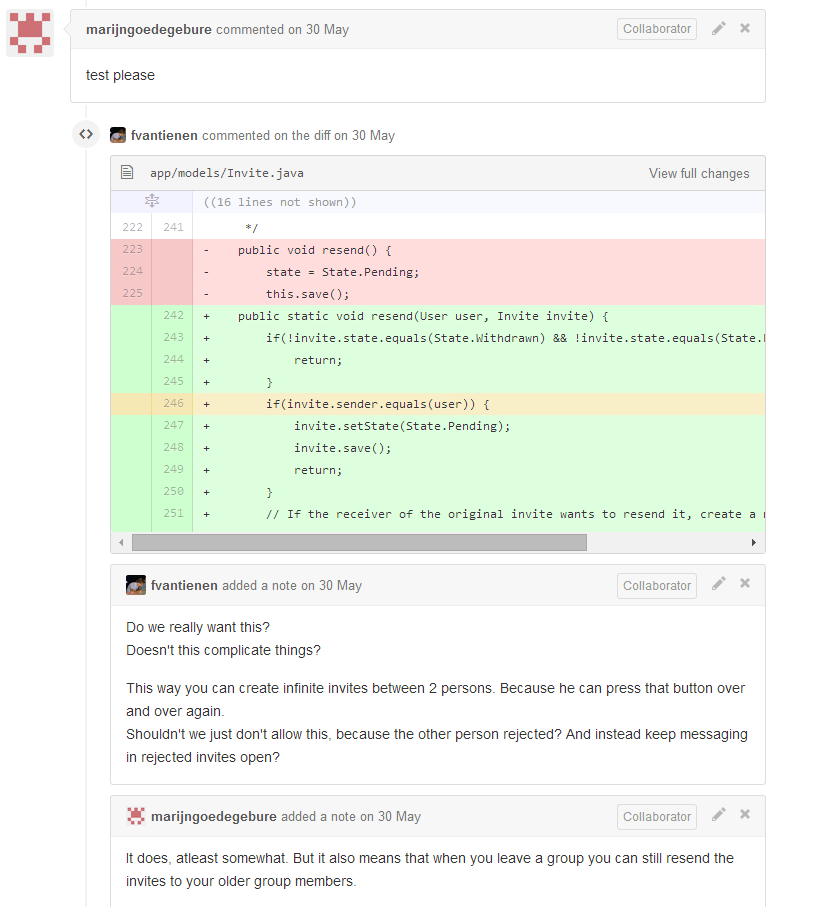
\includegraphics[width=\textwidth]{images/pullrequest-example1}
    \caption{An example of a pull request comment and reply.}
    \label{pullrequest-example}
\end{figure}

For an overview of the pull request and the comments that were made, you can find more information on the following website:
https://github.com/florisverburg/pm-impl/pulls

\section{Testing methods after the implementation phase}
The testing of the entire system is done after the implementation phase has been completed.
This is partly done by checking if the final product matches the requirements set.
It is also done by letting the target audience use the system and document the findings.
We will start with describing the user tests.

\subsection{User test}
The purpose of the user test is to test the system without the limiting factors of a development environment.
The system will be tested for his robustness in the different kinds of input a user can generate.
The test also let's the user make extensive use of the interface that we provided.
Any errors will be revealed by the user interaction.
If the tester find anything unclear he can comment on that in the appropriate text boxes provided in the survey.

To test the system we will be defining the people that are valid testing subjects and how we documented the various aspects of the test.

\subsubsection{The user}
We define a valid subject for our user test as a person that is part of the target audience (which we already defined in an earlier chapter).
The user should also be unfamiliar with the system.
We will focus our user test on the students, since they will be the biggest group of users of the system.

\subsubsection{The test}
The user will be asked to test different functionalities which we will define beforehand.
The functionalities that are included in the survey for testing are the following:
\begin{itemize}
\item Registration
\item Logging in
\item Register to practical using url
\item Viewing the practical that they registered to
\item Invite other student to join your practical group
\end{itemize}
We hand the user a document which lists the different actions that we want the user to do.
Before and after the test we let the user fill in a survey.
The survey at the start is about who the user is and the survey at the end is about what they thought of the system.
To easily process the responses that we receive, we have used a google form.
In this google form we have combined the survey and the step by step action plan for the tester.
The google form document can be found in the appendix.


\subsubsection{The user test results}
TODO list the different conclusions of the survey

\subsection{Requirements test}
TODO list the different requirements that have been met and say something about the progress made.

\section{Software Improvement Group Feedback}
\subsection{Intermediate feedback}
\subsection{Improvements}
\subsection{Final feedback}


